% Created 2024-11-18 Mon 20:14
% Intended LaTeX compiler: pdflatex
\documentclass[11pt]{article}
\input{../../../preamble.tex}
% setting up title page
\title{
  
\includegraphics[width=0.4\textwidth]{fmf_logo}\\
  {\small Oddelek za fiziko} \\
  {Osnove mikrovalovne tehnike}\\
  {\small Poročilo pri FP5}\\

}
\date{}
\author{ Kristofer Č. Povšič, 28211104 \\[5 cm]
 \small  Asistent: Tilen Knaflič \\
}
\addbibresource{refs.bib}


\begin{document}

\maketitle
\newpage
\tableofcontents

\setcounter{page}{2}
\section{Uvod}\label{sec:org9f570f6}

Mikrovalovi so elektromagnetno valovanje z valovno dolžino nekaj centimetrov in frekvenco nekaj GHz. Kot izvor mikrovalov služijo klistroni (ang. \emph{klystron}) in se ga uporablja za ojačitev visokih radijskih frekvenc - od UHF (ultra-high frequencies) do mikrovalov.

\begin{slika}[H]
  \begin{center}
    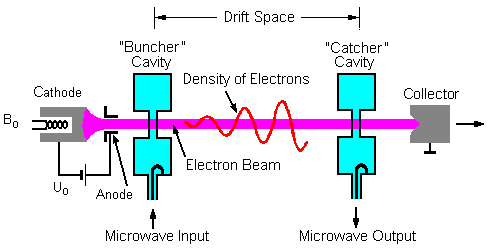
\includegraphics[width=.9\linewidth]{./figures/Klystron}
    \caption{\small Shema enega izmed vrst klistronov. Vir: \cite{noauthor_klystron_2024}}\label{fig:1}
  \end{center}
\end{slika}


Resonančne votline (ang. \emph{cavity resonators}) so v klistronu uporabljene zato, da dodajo signal elektronskemu curku in odstranijo ojačan signal iz njega. Lastno nihanje elektromagnetnega polja v resonančni votlini ustvarja med mrežicama izmenično napetost, ki enakomerni curek elektronov hitrostno modulira. Zaradi tega nastanejo zgoščine in razredčine v elektronskem curku.

Na sliki se nahaja najenostavnejši klistron z dvema resonančnima votlinama. V navodilih za vajo se preseku elektronskega curka in črnih črt resonančnih votlin reče ``mrežica''.

V refleksnem klistronu je na mestu kolektorja odbojna elektroda, ki neenakomerni elektronski curek usmeri nazaj proti resonančnima votlinama in katodi. Ob pravilno izbrani odbojni napetosti se vračajoči curek vrne med mrežico s tako fazo, da električno polje gruč elektronov ojači lastno nihanje elektromagnetnega polja v resonančni votlini in klistron deluje kot oscilator.

Ta pogoj za pozitivno povratno zvezo deluje pri več diskretnih vrednostih napetosti: reče se, da klistron deluje v različnih rodovih.

Mikrovalovno elektromagnetno polje iz resonančne votline speljemo v valovod, kar je vodnik v obliki dveh vzporednih žic, kablov ali cevi namenjen za strogo usmerjeno prenašanje mikrovalov.

Značilna in lahko merljiva količina za stojno valovanje v vodniku je razmerje med minimalno in maksimalno amplitudo napetosti ali toka, ki ga imenujemo ubranost

\begin{equation}
\label{eq:1}
s = \frac{\left| U_{min} \right|}{\left| U_{max} \right|} = \sqrt{\frac{h_{min}}{h_{max}}}
\end{equation}

Reaktanco bremena \(\eta_R\) normirano na karakteristično upornost lahko zapišemo kot

\begin{equation}
\label{eq:2}
\frac{\eta_R}{Z_0} = \frac{(s ^2 - 1) \tan (\beta x_{min})}{1 + s ^2 \tan ^2(\beta x_{min})}
\end{equation}

kjer \(x_{min}\) določimo z dvojno meritvijo:

\begin{enumerate}
\item najprej izmerimo krivuljo ubranosti za vodnik, ki je zaključen z bremenom,
\item nato pa še za vodnik, ki je kratko sklenjen
\end{enumerate}

in fazna konstanta je  \(\beta = \omega \sqrt{LC}\).
Pri kratko sklenjenem vodniku je \(U_{min} = 0\) pri \(x = 0\), pri vodniku
zaključenem z bremenom, pa različen od 0, se opazovani minimum ubranosti
premakne proti bremenu ravno za vrednost \(x_{min}\).


Enaka normirana rezistenca pa je

\begin{equation}
\label{eq:3}
\frac{\xi_R}{Z_0} = (1 - \frac{\eta_R}{Z_0} \tan \left(\beta x_{min}\right))s
\end{equation}

Frekvenco mikrovalov lahko merimo z resonatorjem, ki ga ugradimo v valovod.
Umerimo ga s premikanjem dna. Ko je uglašen se tudi v njem pojavi valovanje tako,
da se del moči valovanja na valovodu porabi (za \(60\%\)). Če je vijak umerjen v
frekvenčni skali lahko hitro določimo frekvenco valovanja v valovodu.

Moč merimo najpogosteje s termoelektričnimi elementi, ki se zaradi obsevanja močno segrejejo in se jim zato spremeni upornost. Takim elementom pravimo bolometri. Če z njim izmerimo moč \(P_m\) dobimo celotno vpadno moč kot

\begin{equation}
\label{eq:4}
P = \frac{P_m}{1 - \left| r_R \right| ^2}; \quad \left| r_R \right|^2 = (\frac{1 - s}{1 + s}) ^2
\end{equation}

Termistorji so izdelani iz polprevodnikov, ki so pomešani z bakrenim prahom za boljšo prevodnost. Zveza med močjo in spremembo upornosti ni popolnoma linearna za razliko od bareterjev, ki so iz tanke platinaste žičke. Slednji so občutljivi na preobremenitve, kar termistorji niso.
\section{Potrebščine}\label{sec:org0f556ee}
\begin{itemize}
\item klistron
\item ubiralka
\item dušilka
\item resonator
\item merilni vod
\item kratkostična stena
\item antena
\item bolometer
\item osciloskop in voltmeter
\end{itemize}
\section{Naloge}\label{sec:orgc5da1f2}
\begin{itemize}
\item prilagodite valovod na generator mikrovalov
\item izmerite frekvenco valovanja s pomočjo resonatorja
\item posnemite rodove klinstronovega delovanja v odvisnosti od odbojne napetosti
\item izmerite moči, ki jih porablja termistor v vrhovih najmočnejših rodov
\item z osciloskom posnemite krivulji ubranost za valovod, ki je zaključen z bremenom in za kratko sklenjeni valovod.
\end{itemize}
\section{Obdelava podatkov in izračuni}\label{sec:orgb6430b5}

Podatke sem shranil v .csv format in jih obdelal s pomočjo programerskega
jezika Python in knjižnic matplotlib, pandas, numpy, cmasher ter
uncertainties.
\subsection{Frekvenca mikrovalov}\label{sec:orgb9f4d6a}

Frekvenco sem izmeril z uglaševanjem resonatorja vgrajenega v valovod. Pri
meritvi lege vijaka sem dobil vrednost \(414\), iz česar po umeritveni
krivulji \ref{slika} sledi, da je frekvenca mikrovalov

\[ \nu = (8.43 \pm 0.01) \mathrm{GHz}
\]

\begin{slika}[H]
\begin{center}
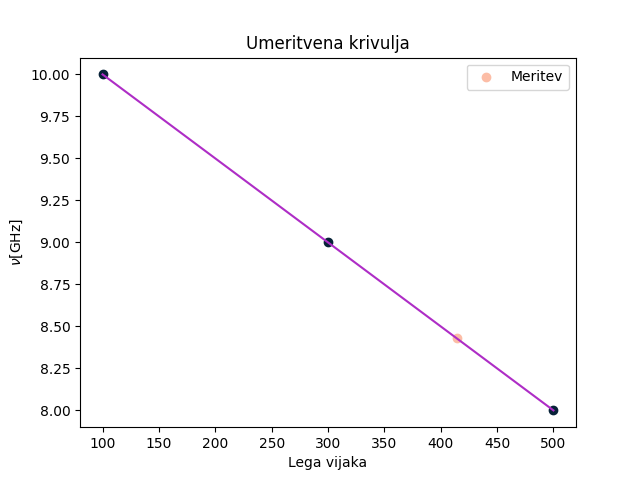
\includegraphics[width=.9\linewidth]{/mnt/Data/02AreasLenovo/Sola/FMF/2letnik/1semester/FP5/04mikroval/figures/umeritev.png}
\end{center}
\caption{\small Graf umeritve za frekvenco. }\label{fig:umeritev}
\end{slika}


\subsection{Meritve ubranosti}\label{sec:org4464617}

Z drsnim merilnikom sem lahko izmeril stoječe valovanje, kakor se vidi na
slikah \ref{fig:zajem_signala}, \ref{fig:krivulja_ubranosti}. Označene so tudi
odčitane vrednosti, iz
katerih sem po enačbi \ref{eq:1} potem izračunal ubranost, ki je za bolometer
znašala:

\[s = 0.443 \pm 0.006
\]

\begin{slika}[H]
\begin{center}
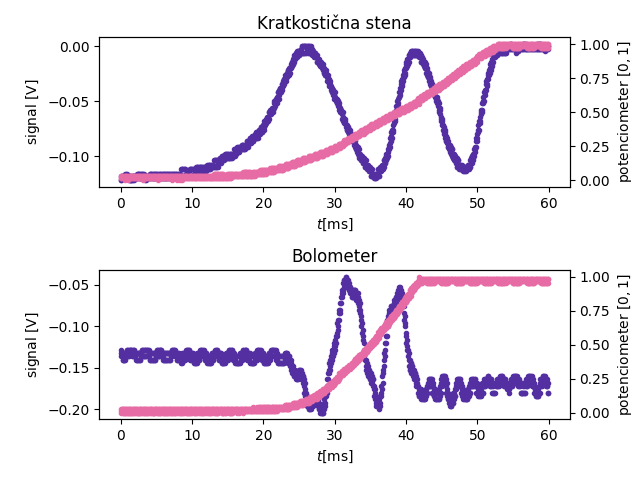
\includegraphics[width=.9\linewidth]{figures/kratkoInBolo}
\end{center}
\caption{\small Graf prikazuje zajem signala, kakor je izgledal na osciloskupo}\label{fig:zajem_signala}
\end{slika}

\begin{slika}[H]
\begin{center}
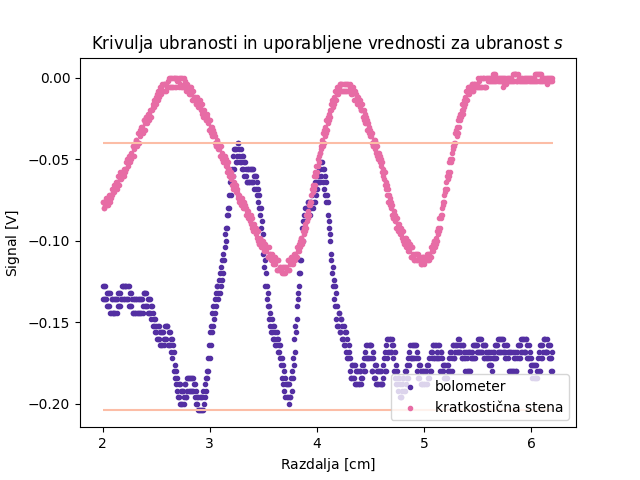
\includegraphics[width=.9\linewidth]{/mnt/Data/02AreasLenovo/Sola/FMF/2letnik/1semester/FP5/04mikroval/figures/krivulja_ubranosti.png}
\end{center}
\caption{\small Graf prikazuje krivuljo ubranosti z označenim odbranim maksimumom
in minimumom}\label{fig:krivulja_ubranosti}
\end{slika}

Za kratkostično steno je po navodilih ubranost enaka 0.

Razdalja med dvema minima na krivulji, ki opisuje kratkosklenjen valovod,
je enaka polovici valovne dolžine valovnja v valovodu. Odčitane vrednosti so
na sliki \ref{fig:x_min}. Dobim:

\[ \lambda' = (2.58 \pm 0.02) \mathrm{cm}
\]

\begin{slika}[H]
\begin{center}
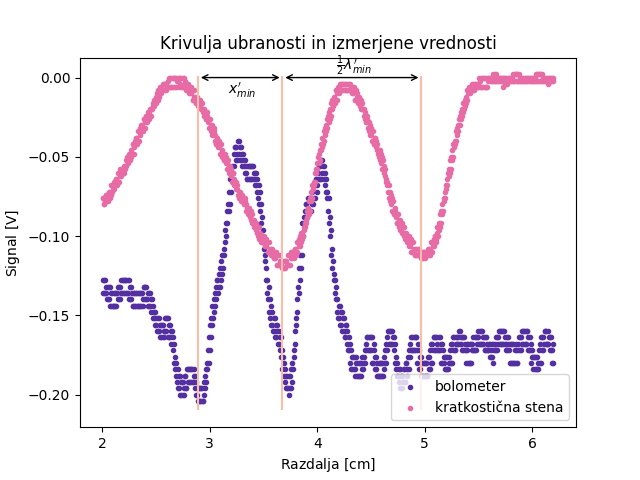
\includegraphics[width=.9\linewidth]{figures/krivulja_ubranosti_x_min}
\end{center}
\caption{\small Graf prikazuje krivuljo ubranosti z označenim odbranimi vrednostmi
  za \(x_{min}'\) in \( \lambda'\).}\label{fig:x_min}
\end{slika}


Razlika med lego izbranega minimuma krivulje, ki opisuje valovod z bremenom
in ustreznega minima krivulje kratko sklenjenega valovoda je \(x_{min}'\).
Odčitane vrednost so na sliki \ref{fig:x_min}.

Izmeril sem

\[ x_{min}' = (0.78 \pm 0.1) \mathrm{cm}
\]

Velja

\begin{equation}
\label{eq:5}
\frac{x_{min}' }{\lambda'} = \frac{\beta x_{min}}{2 \pi}
\end{equation}

saj je dano razmerje količin enako v vakuumu in znotraj valovoda.

Iz dane enačbe tako dobimo vrednost

\[ \beta x_{min} = 1.91 \pm 0.01
\]


Sedaj lahko po enačbah \ref{eq:2} in \ref{eq:3} izračunamo relativno reaktanco
bremena

\[ \frac{\eta_R}{Z_0} = 0.88 \pm 0.3
\]

ter relativno rezistenco

\[ \frac{\xi_R}{Z_0} = 1.55 \pm 0.08
\]

Refleksijski koeficient dan po enačbi \ref{eq:4} ima za bolometer vrednost

\[ \left| r_R \right| ^2 = 0.149 \pm 0.004
\]

s katerim izračunamo pravo moč valovanja \(P\) in izračunane vrednosti
so podane v tabeli \ref{tab:rodovi}.

\begin{tabela}
  \centering
\[
  \begin{array}{|c|c|c|c|}\hline
    U_{0}\  [\mathrm{V}] & P_{m} \ [\mathrm{mW}] \pm 0.01 & P \ [\mathrm{mW}] & P_{err} * 10^{-3} \\ \hline
-29.43 & 0.65 & 0.76 & \pm 1 \\
-47.54 & 0.80 & 0.94 & \pm 1 \\
-54.44 & 1.50 & 1.76 & \pm 1 \\
-82.10 & 1.75 & 2.06 & \pm 1 \\
-92.40 & 2.90 & 3.41 & \pm 2 \\
-133.00 & 3.30 & 3.88 & \pm 2 \\
-146.80 & 4.80 & 5.64 & \pm 3 \\
-230.80 & 5.65 & 6.64 & \pm 3 \\
-339.60 & 3.70 & 4.35 & \pm 2 \\
-367.90 & 3.40 & 4.00 & \pm 2 \\\hline
    \end{array}
\]
\caption{\small Tabela prikazuje izmerjene in izračunane vrednosti. Po vrsti:
napetost rodovov, izmerjene moči, prava moč in napaka prave moči.}\label{tab:rodovi}
\end{tabela}

\nocite{*}
\printbibliography[heading=bibintoc]

\end{document}
